\chapter{Fussballszenario} \label{kap:Fussballszenario} %TODO: Besseren Kapiteltitel

\section{Szenario Koordination}  %TODO: Hendrik
\sectionauthor{H.O.}

Die Szenario Koordination umfasst sowohl das Verhalten der einzelnen AMiRos, kooperative Elemente zwischen verschiedenen AMiRos als auch die Kommunikation mit dem Host-PC. Der Entwurf dieser drei Themenbereiche sollen im folgenden kurz vorgestellt und begründet werden:\\
Um ein bestimmtes Verhalten zu zeigen, müssen die AMiRos selbst zunächst über einen Satz einzelner Fähigkeiten verfügen. Ein komplexeres Verhalten entsteht dann aus der Kombination der einzelnen Fähigkeiten, indem diese sequenziell oder parallel miteinander kombiniert werden. Denkbar wäre ebenso die Realisierung einer Verhaltenshierarchie, in der sich einzelne Verhaltensweisen beeinflussen und sich gegenseitig unterdrücken oder verstärken können. Ein solcher Ansatz wird näher in \cite{Brooks:1986} beschrieben.\\
Da das Szenario in seiner Komplexität jedoch noch begrenzt ist und kein vollständig generisches Verhalten implementiert werden musste, wurde für die Umsetzung im Projektkontext durch eine einfache State-Machine realisiert. Die Zustände stellen einzelne Verhaltensweisen des Roboters dar und durch bestimmte Nachrichten (Events) kann zwischen ihnen gewechselt werden.\\
Das Verhalten einzelner AMiRos wird erweitert durch kooperative Fähigkeiten und die Möglichkeit der Kommunikation durch einen festgelegten Befehlssatz. Kann beispielsweise ein AMiRo während einer Spielaktion den Ball nicht lokalisieren, kann er eine Nachricht an den anderen AMiRo schicken, woraufhin dieser sich dann ein Stück bewegt, um die Sicht auf den Ball freizugeben.\\
Zusätzlich besteht die Möglichkeit für die AMiRos mit dem Host-PC zu kommunizieren, der an Hand eines Kamerabildes und zusätzlicher Bildverarbeitungslogik das Spielgeschehen verfolgen, interpretieren und steuern kann. Dies erlaubt außerdem eine Benutzerinteraktion um das Spiel zu starten, zu pausieren oder zu unterbrechen. In der derzeitigen Realisierung übermittelt der Host-PC außerdem noch den Status des Spielballs, also ob dieser in Bewegung ist oder ruht. Diese Information wird von den AMiRos verwendet, um eigenständig zu bestimmen, welcher AMiRo gerade am Zug ist.

\vfill

\subsection{Kommunikation per RSB und Spread} %TODO: Hendrik
Damit die AMiRos untereinander kommunizieren können, wurde eine Publish-Subscribe Architektur basierend auf der RSB Middleware aufgesetzt und anstatt einer einfachen Socket-Transport Lösung wurde auf das etwas komplexere Spread Toolkit zurückgegriffen (siehe RSB Konfigurationsdatei im Anhang \ref{sec:rsb-config}).\\
Die Publish-Subscribe Architektur bietet den Vorteil der asynchronen Kommunikation, die im Zusammenspiel mit einer State-Machine besonders praktisch ist. Die State-Machine muss nicht auf explizit auf Antworten warten, sondern kann beliebig weiterlaufen und reagiert erst dann, wenn eine Nachricht empfangen wurde. Zudem bietet sie den Vorteil das sehr leicht Software-Komponenten hinzugefügt und an die bestehende Kommunikation angeschlossen werden können (vgl.\cite{Siciliano:2007}).\\
Jeder AMiRo (und auch der Host-PC) hat also eine bestimmte Anzahl an Empfängern (Listener) und Sendern (Publisher) um Nachrichten in bestimmten Geltungsbereichen (Scopes) zu empfangen oder zu senden.\\%TODO:RSB Literatur Verweis?
Das Spread Toolkit hilft dabei einen Nachteil der allgemeinen Publish-Subscriber Architektur zu beseitigen: Die Kommunikation beruht nicht auf einem zentralen Endpunkt, der die gesamte Kommunikation steuert, sondern jeder Spread-Daemon überwacht die Verbindungen zu allen anderen Endpunkten und hält diese so aufrecht (vgl.\cite{Siciliano:2007}). So kann auch bei kurzzeitigen Verbindungsabbrüchen sichergestellt werden, dass die Verbindung automatisch wiederhergestellt wird. Auf Programmebene  muss so weniger Overhead für die Sicherstellung der Verbindung implementiert werden und der Code bleibt einfacher und somit besser wartbar.\\
Neben der Plattform-übergreifenden Kommunikation werden RSB und Spread zusätzlich auch für Interprozess-Kommunikation auf den AMiRos und auf dem Host-PC eingesetzt. Wie in Abb. \ref{fig:spread} zu sehen ist, laufen auf beiden AMiRos die drei gleichen Softwarekomponenten. Die State-Machine (FSM) steuert das Verhalten und die Kommunikation. Die locateAndShoot Komponente stellt die Verhaltenseinheiten für das Szenario zur Verfügung und die SearchCharging Komponente erlaubt aus dem Szenario aus die Lokalisation und das Anfahren an die Ladestation. Diese drei Komponenten kommunizieren über den internen Spread, der auf der internen localhost Schnittstelle auf dem Port 4806 läuft (siehe dazu auch Anhang \ref{sec:spread-config}).\\
Die Kommunikation zwischen den AMiRos selbst und dem Host läuft über einen weiteren Spread-Daemon, der mit einer anderen Konfiguration geladen wird, die W-LAN Schnittstelle nutzt und auf Port  4803 hört und sendet (siehe ebenfalls Abschnitt \ref{sec:spread-config}).\\
Die W-LAN Verbindung wurde durch einen eigenen Router realisiert und erlaubt so die feste Adresszuweisung für die drei Endpunkte, damit die Spread-Konfiguration darauf zurückgreifen kann. Die Einzelheiten können der W-LAN Konfiguration im Anhang (\ref{sec:wlan-config}) entnommen werden.
\begin{figure}[H]
	\begin{center}
		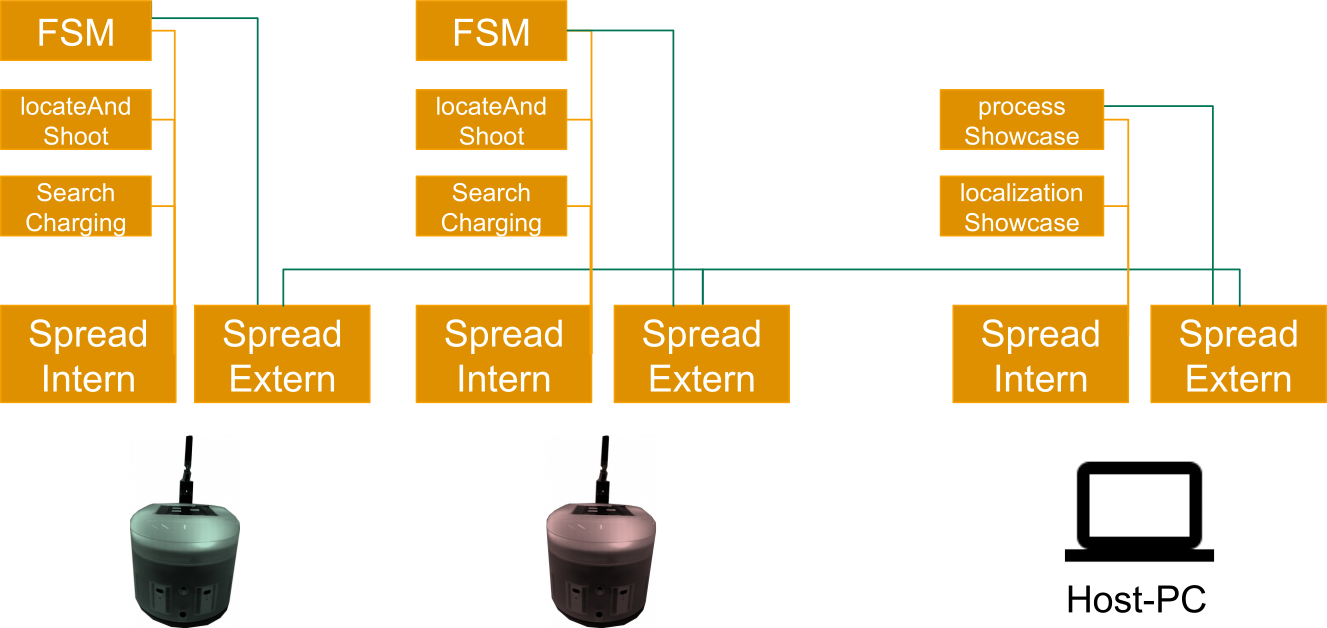
\includegraphics[scale=.65]{spread_communication.png} 	
		\caption{Spread-Kommunikation}
		\label{fig:spread}
	\end{center}
\end{figure}

\subsection{Finite-State-Machine} %TODO: Hendrik
Die State-Machine regelt das Verhalten der einzelnen AMiRos. Jedes Verhalten wird in kleinstmögliche Einheiten unterteilt, die dann einzeln angesprochen und überall wiederverwendet werden können. Nach der Initialisierung aller RSB-Komponenten und Variablen wird im Programm die State-Machine gestartet.\\ 
Solange kein Fehler auftritt, bleibt das Programm immer in der State-Machine und wechselt den aktuellen Zustand nur auf Grund externer Nachrichten, die durch in Form von RSB Events oder CAN Messages eingehen können. Extern beschreibt also in diesem Zusammenhang sowohl die anderen Programmkomponenten die auf dem AMiRo laufen, als auch RSB Events von einem anderen AMiRo oder dem Host-PC und CAN Nachrichten vom Mikrocontroller.\\
Einzelne Zustände haben auch direkte Anweisungen die den aktuellen Zustand wechseln können, diese soll eine Kapselung der einzelnen Verhaltenseinheiten unterstützen und erlaubt zukünftige Änderungen oder Erweiterungen leichter durchführen zu können.\\
Die State-Machine selbst ist in Abb. \ref{fig:fsm-amiro} dargestellt. Nach dem Start ist zunächst der Idle-Zustand aktiv. Dieser wartet lediglich auf Kommandos und stellt sicher, dass sich der AMiRo nicht bewegt, sondern ruhig auf seiner Position abwartet.\\
Wird das Spiel dann gestartet, wechselt der aktuelle Zustand auf startScenario.
\begin{figure}[H]
	\begin{center}
		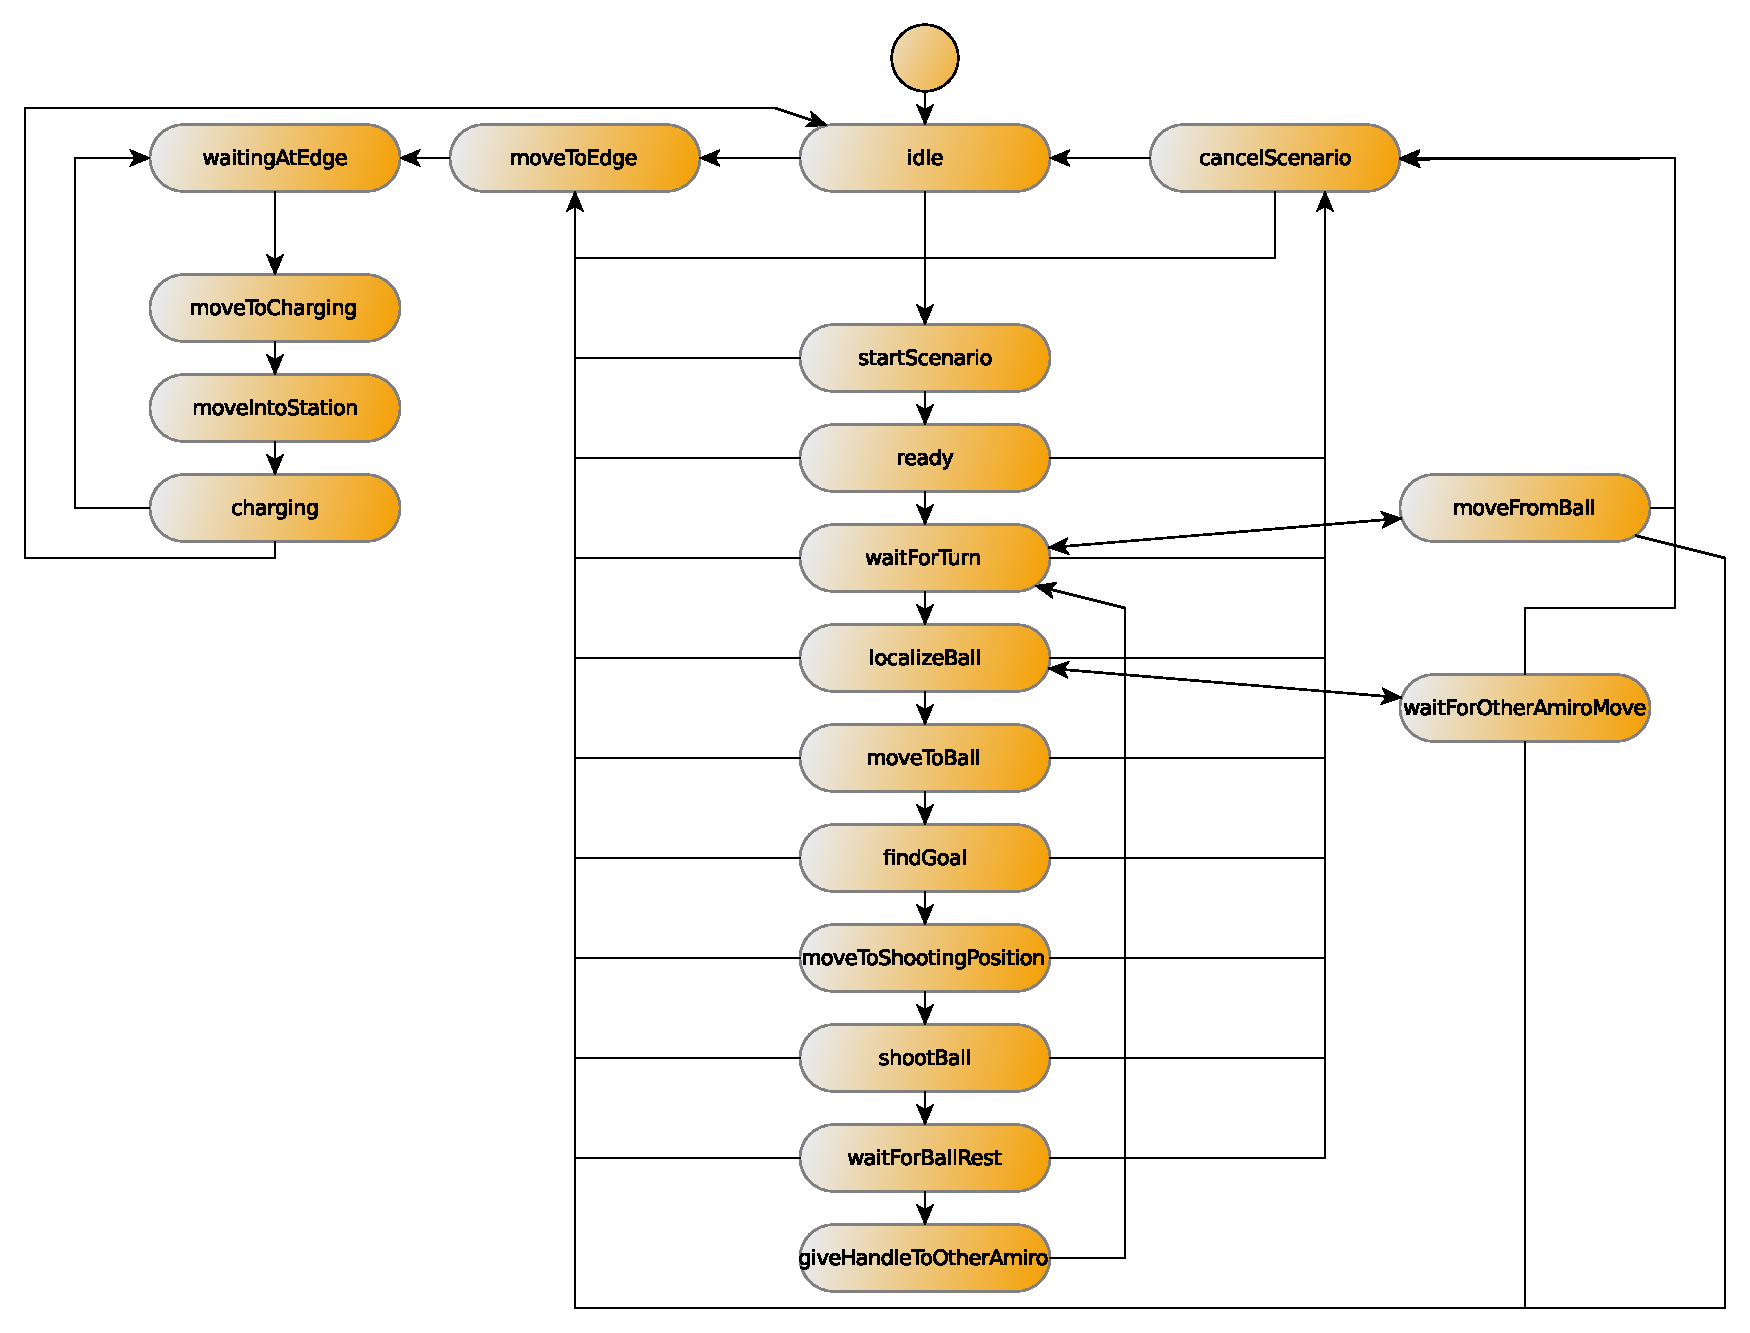
\includegraphics[scale=.55]{Final_FSM_AMiRo.pdf} 	
		\caption{Finite-State-Machine}
		\label{fig:fsm-amiro}
	\end{center}
\end{figure}

\section{Realisierung der einzelnen Spielelemente} %TODO: Besseren Sectiontitel

\subsection{Lokalisation des Balls} %TODO: Julian E.

\subsection{Anfahren des Balls} %TODO: Julian E.

\subsection{Lokalisation des gegnerischen Tores} %TODO: Timo M.
- Rotation um eigene Achse zur Lokalisation des Tores
- Lokalisation Anhand von Blobb-Detektion 
- Wenn ein einzelner Pfosten im Bild vorhanden ist - bereits gedrehten Winkel + zusätlichen Winkel vom Mittelpunkt des Bildes zum Pfosten speichern
- Wenn beide Pfosten im Bild vorhanden sind - bereits gedrehten Winkel + zusätlichen Winkel vom Mittelpunkt des Bildes zum Tormittelpunkt speichern und Rotation beenden
- Drehung zum Ball durchführen, um diesen wieder vor sich zu haben

\subsection{Schussposition anfahren} %TODO: Timo M.
- Je nach Winkel zum Tor entscheiden, ob der Ball links- oder rechtsseitig umfahren werden soll
- 90$^\circ$ Drehung zu der gegebenen Seite 
- Umfahren des Balles bis vorher berechneter Winkel zum Tor erreicht ist
	- Bei einem Hindernis wird das Umfahren des Balles gestoppt
- 90$^\circ$ Drehung zum Ball
- Überprüfung, ob sowohl Ball als auch das Tor im Bild zu sehen ist 
	- Ist dies der Fall -> feinjustierung der Schussposition 

\subsection{Schießen} %TODO: Timo M.
- Überprüfen der seitlichen vorderen Abstandssensoren ob eine Wand detektiert wird
	- Sollte eine Wand auf einer Seite detektiert werden -> Angedrehter Schuss mit Drehung des AMiRos weg von der Wand
- Schießen des Balles durch kurzes Ansteuern beider Motoren 

\subsection{Beiseite Fahren} %TODO: Julian E. (Besseren Titel suchen^^)

\section{Spieltracking} %TODO: Julian D.

\subsection{Spielfeldbestimmung mit dem AR Toolkit} %TODO: Julian D.

\subsection{Extraktion wichtiger Spielelemente mit Bildverarbeitungsmethoden} %TODO: Julian D.

\subsection{Benutzerinteraktion mit AR Markern} %TODO: Julian D.

\subsection{Spielkoordination} %TODO: Julian D.

\subsection{Grafische Darstellung der Spielstatus} %TODO: Julian D.